\newpage

\section{Sicherungsbereiche}
	Die Sicherung wird in Bewegung immer über die Uhrzeit ausgegeben. Sowohl in Fahrzeugen als auch zu Fuß in Marschformationen.  Die Marschrichtung ist immer 12 Uhr. \\

\subsection{Rundumsicherung}
	 Rundumsicherung bedeutet, dass 360° vom Trupp abgesichert werden. Jeder Soldat hat dazu den Auftrag, ein Viertel des \glqq Kreises\grqq\space abzusichern. Eine Rundumsicherung kann aus dem Marsch oder in einer Stellung vollzogen werden. In einer Stellung geht es nicht darum, einen perfekten Kreis zu bilden – sondern sich in Deckung zu bewegen und von dort aus seinen Sektor zu sichern. Je nach Bedarf kann der Truppführer sich, um z.B. zu funken, eine 4 Mann Sicherung aufbauen lassen. \\
	Standardsicherung  – 4 Mann: 
		\begin{itemize}
			\item Nr.1 sichert auf 12 Uhr 
			\item Nr.2 sichert auf 9 Uhr 
			\item Nr.3 sichert auf 3 Uhr 
			\item Nr.4 sichert auf 6 Uhr 
		\end{itemize}
		\begin{figure}[htbp]
			\centering
			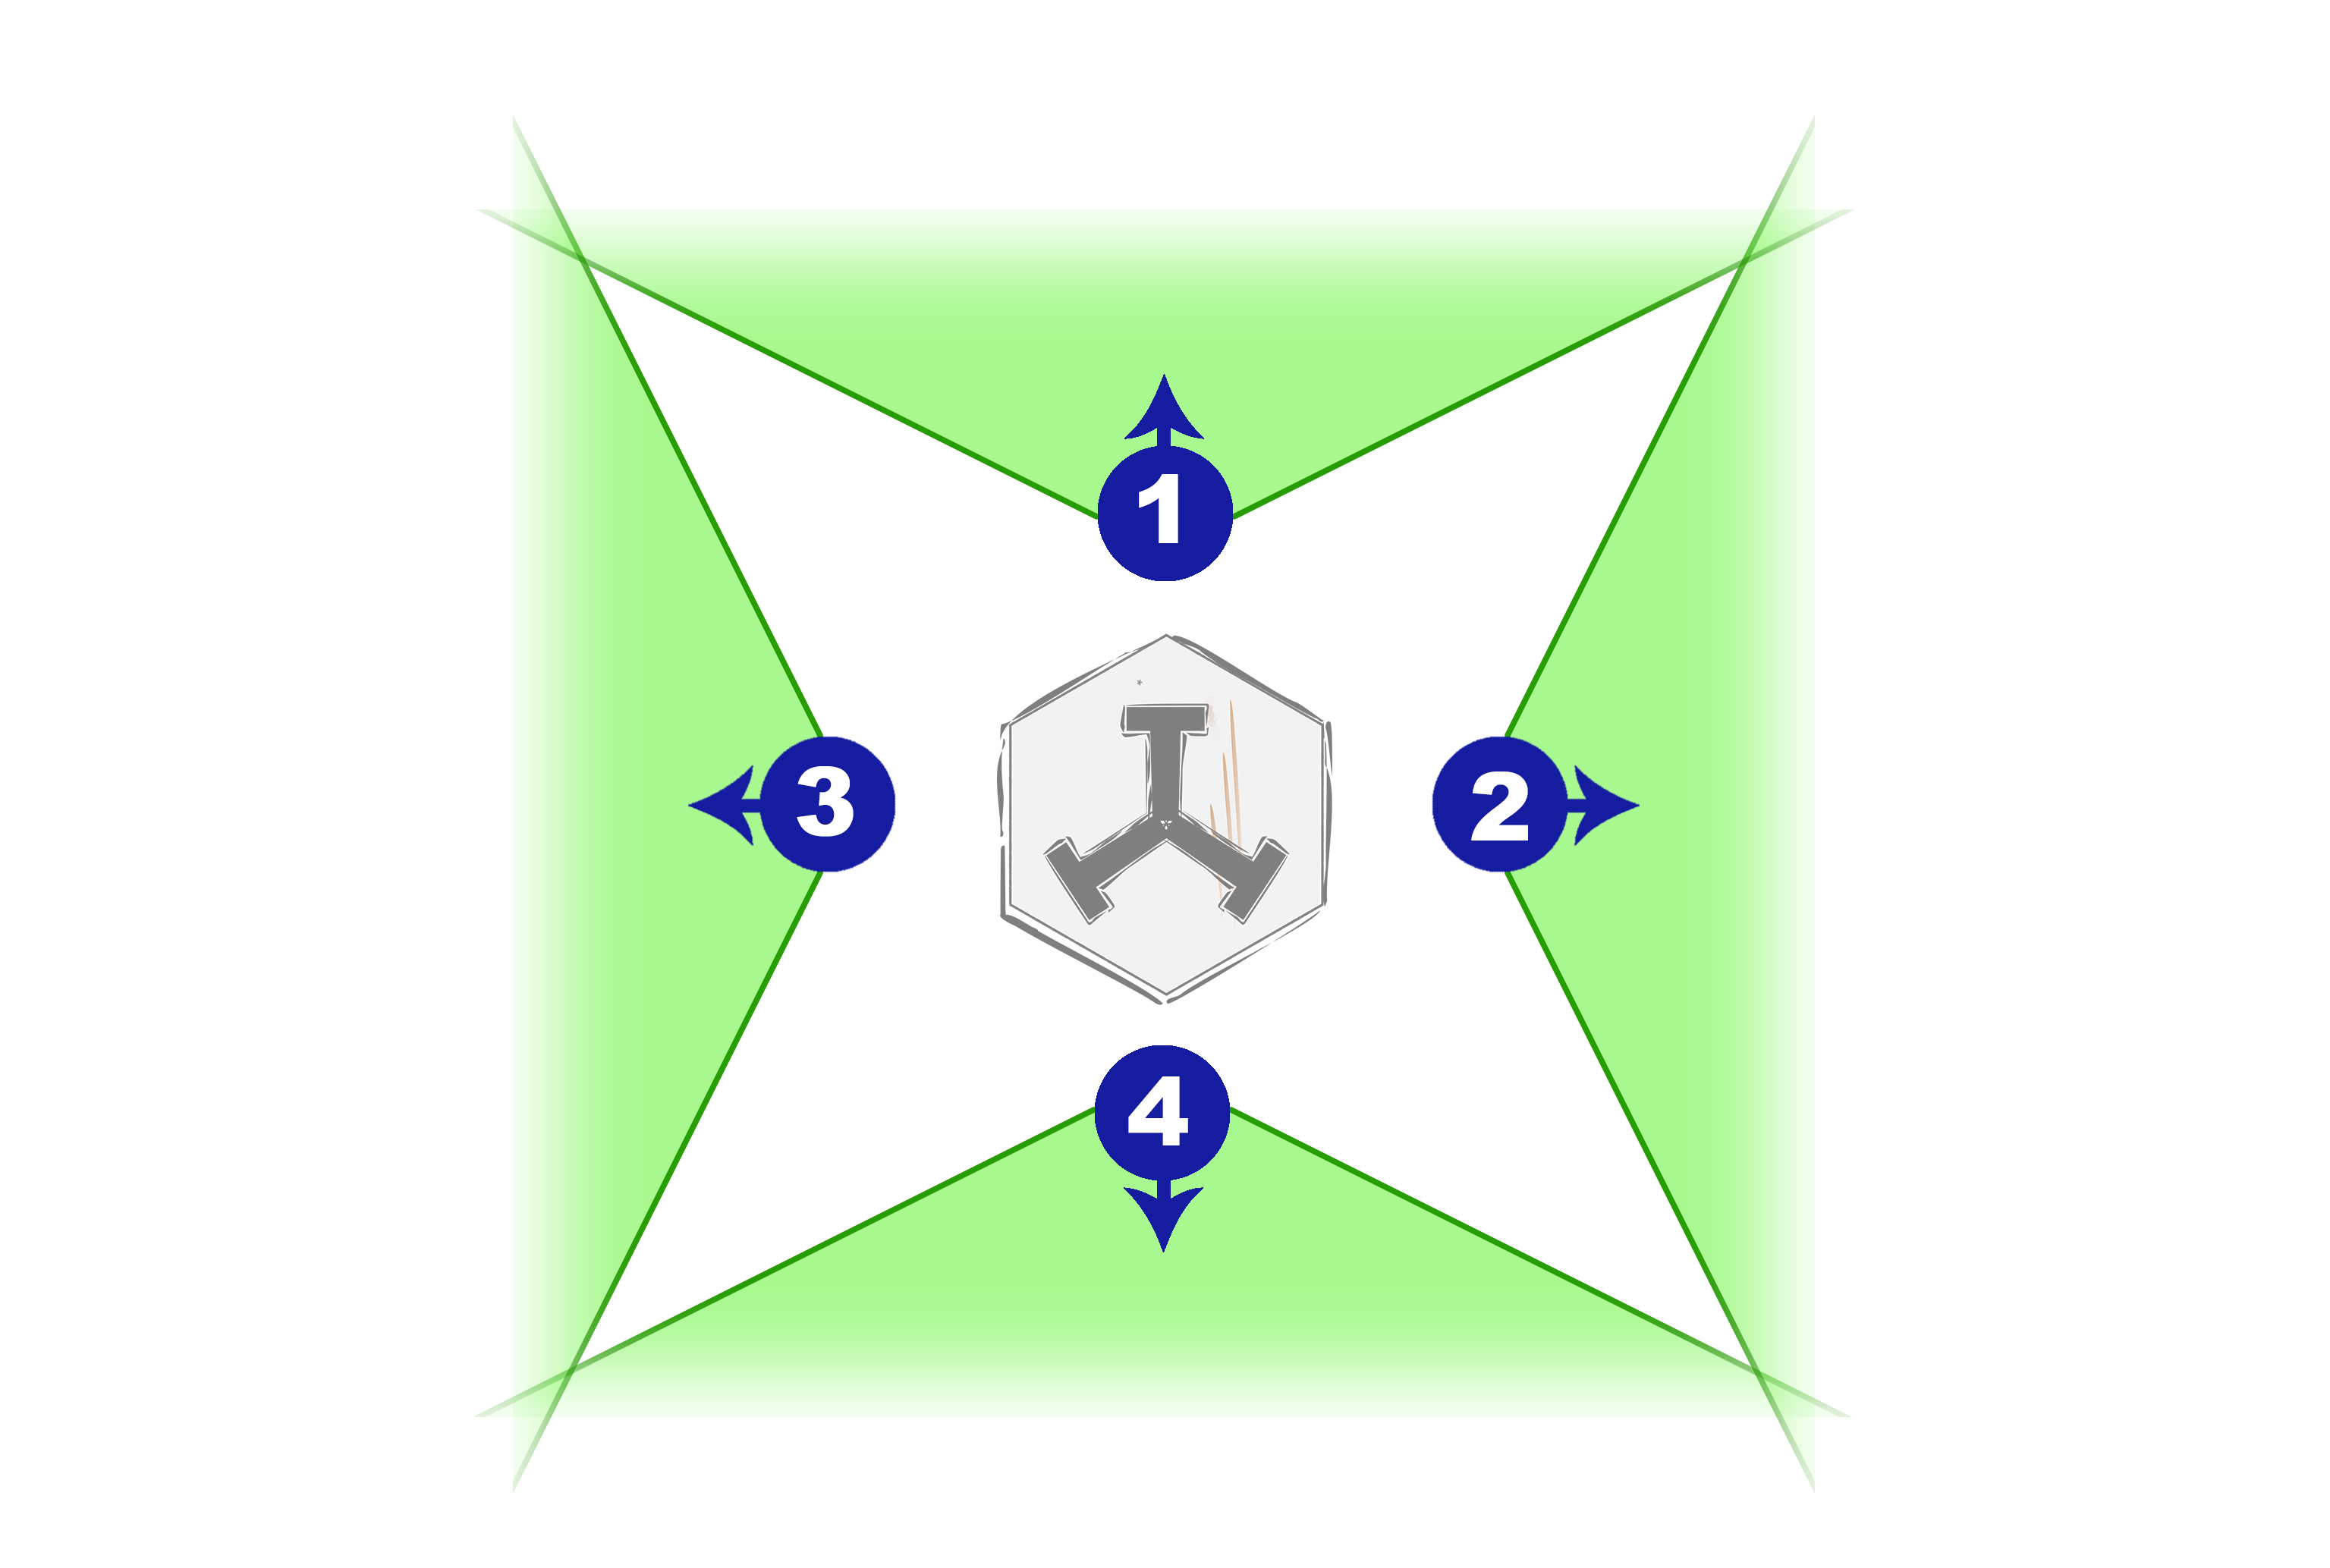
\includegraphics[width=0.8\linewidth]{./img/grundlagen/sicherungen/360grad_sicherung_4mann.jpg}
			\caption{4 Mann 360er}
		\end{figure}

	Standardsicherung – 6 Mann: 
		\begin{itemize}
			\item Nr.1 und Nr. 2 sichern auf 12 Uhr 
			\item Nr.3 sichert auf 3 Uhr 
			\item Nr 4 und 6 sichern auf 6 Uhr
			\item Nr.5 sichert auf 9 Uhr
		\end{itemize}
		\begin{figure}[htbp]
			\centering
			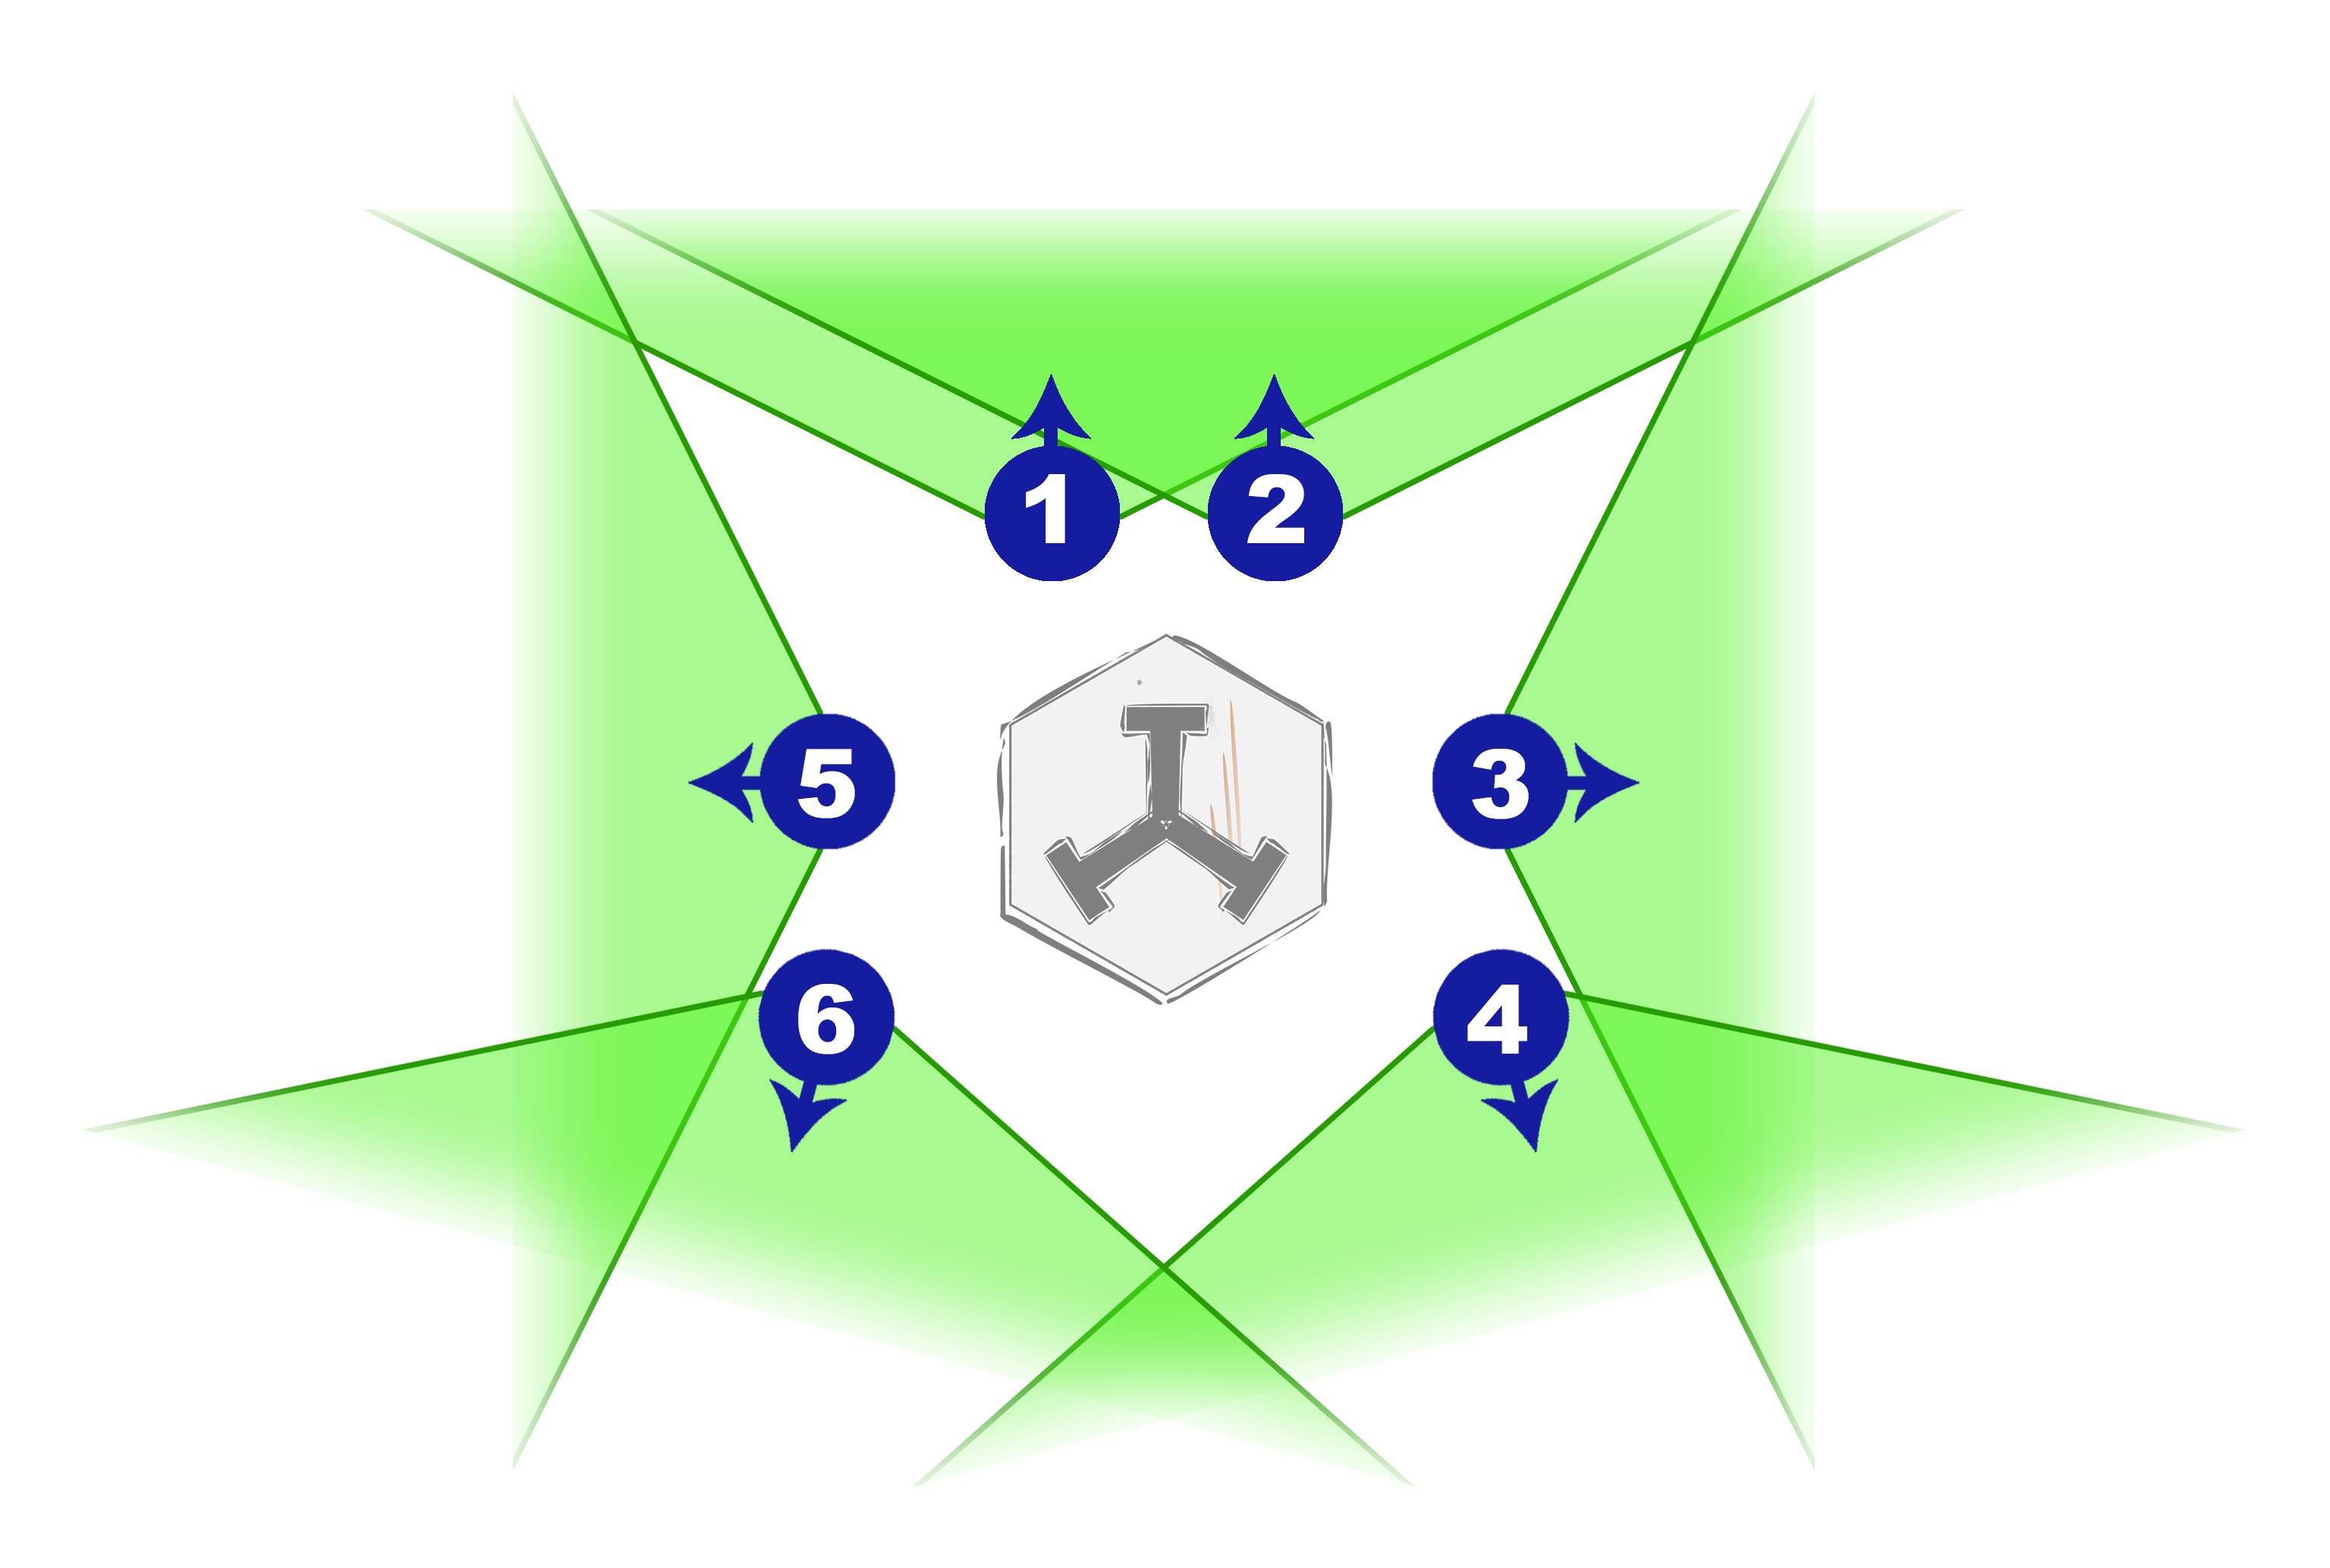
\includegraphics[width=0.8\linewidth]{./img/grundlagen/sicherungen/360grad_sicherung_6mann.jpg}	
			\caption{6 Mann 360er}
		\end{figure}
		

\subsection{180°-Sicherung}
	Die 180-Grad-Sicherung ist eine Halbkreis-Sicherung. Sie wird in der Regel an Mauern angewandt oder in einer Stellung, um ein zu beobachtendes Gelände abzusichern, wenn der Rückraum als absolut sicher gilt. Zu beachten ist, dass die 180° Sicherung nicht unmittelbar an der Mauer sondern etwa 1m entfernt aufgebaut wird. So können einzelne Soldaten oder Trupps hinter der Sicherung kreuzen, ohne in den eigenen Feuerbereich treten zu müssen. \\
	\begin{figure}[htbp]
		\centering
		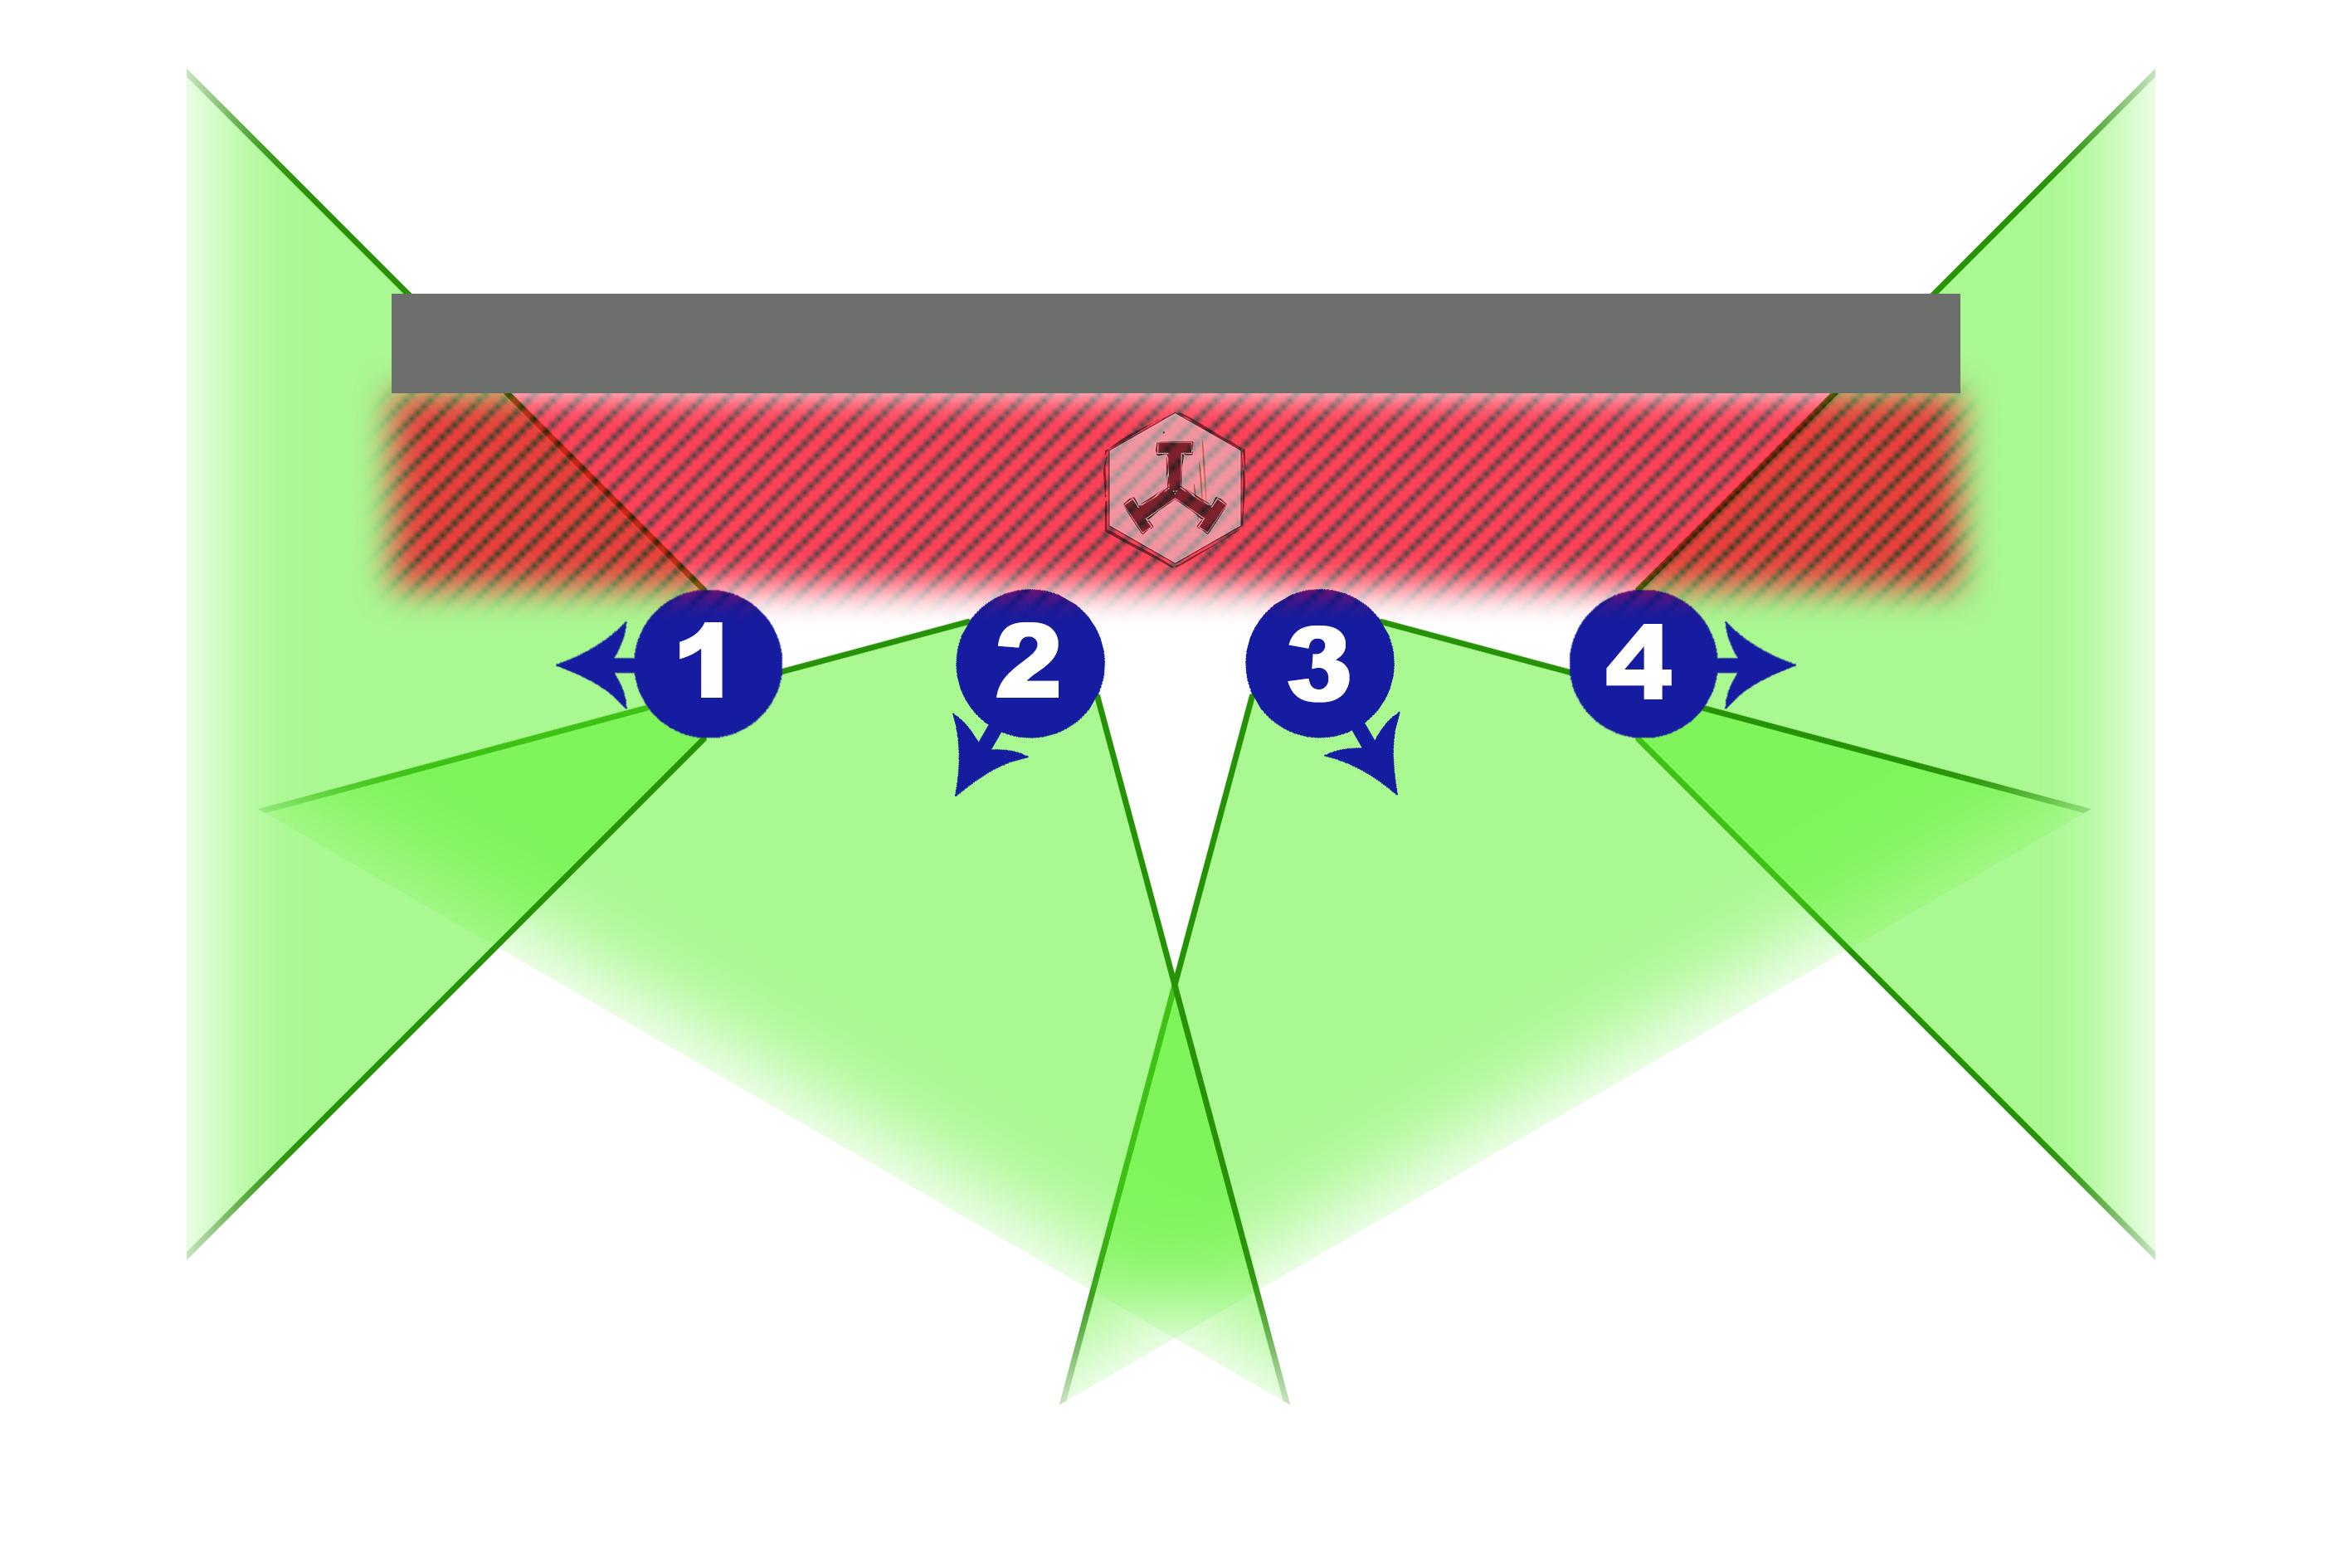
\includegraphics[width=0.8\linewidth]{./img/grundlagen/sicherungen/180grad_sicherung_4mann.jpg}
		\caption{180° Sicherung an Mauer 4 Mann}
		\end{figure}
		
		\begin{figure}[htbp]
			\centering
			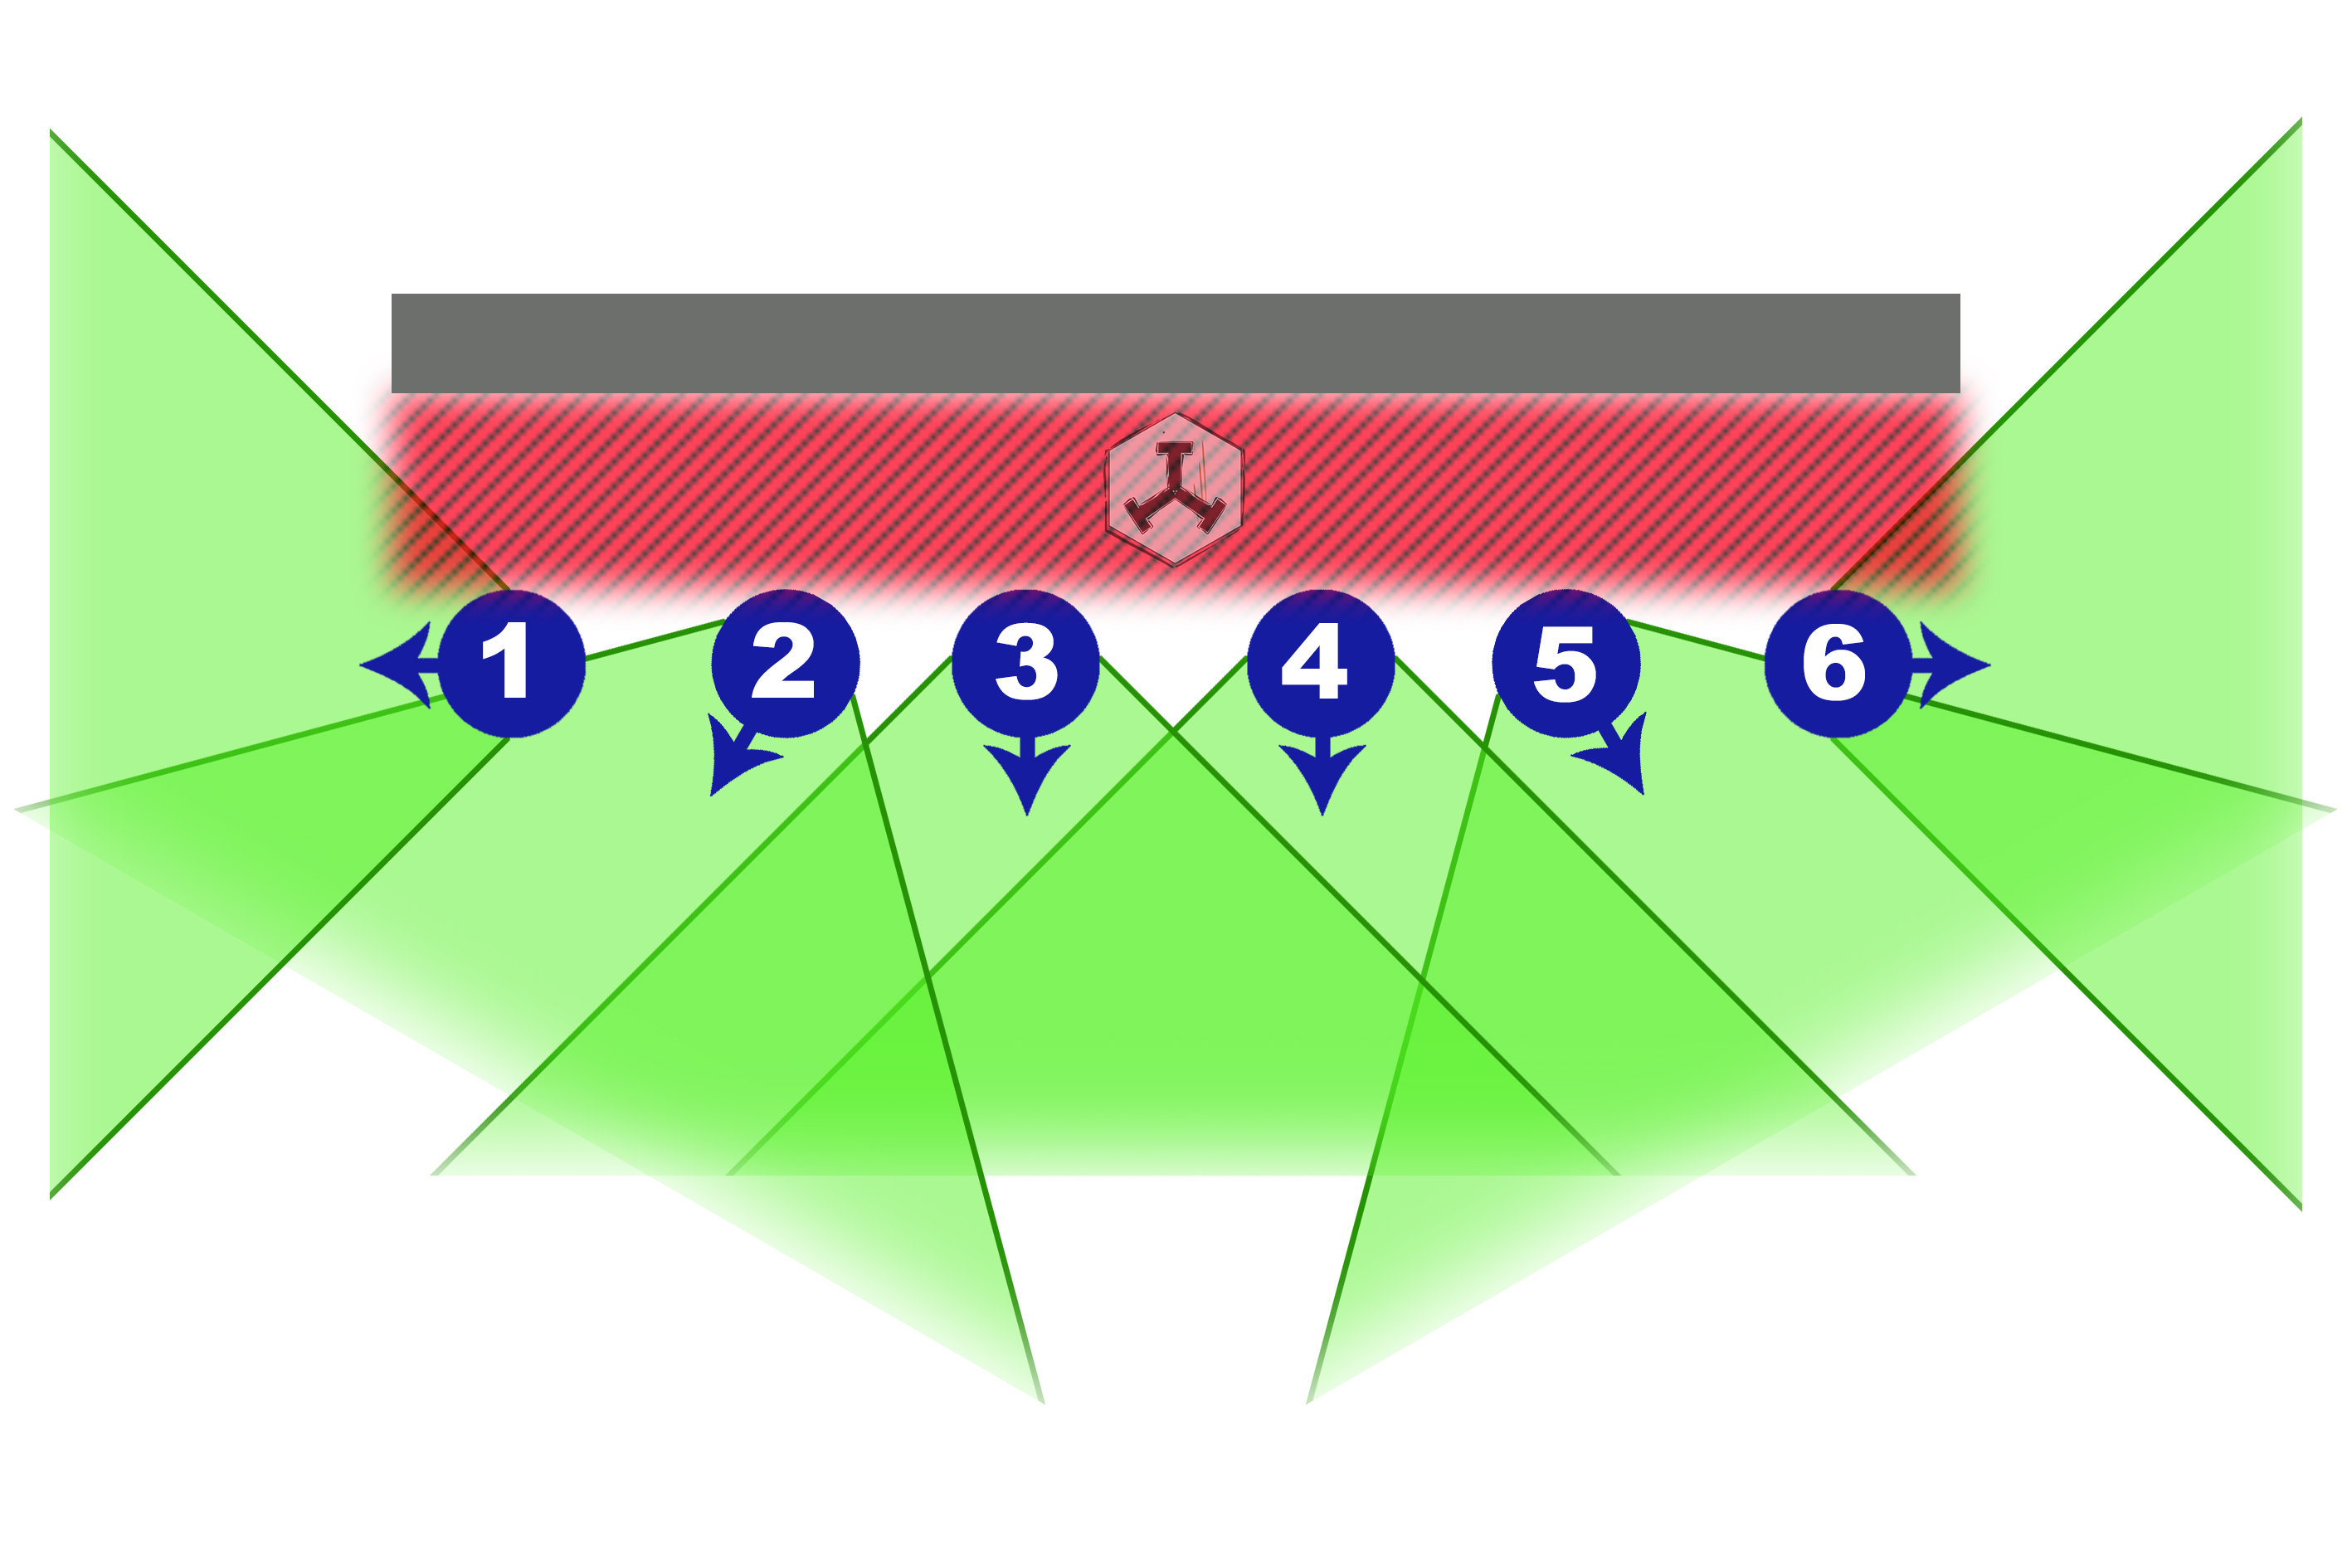
\includegraphics[width=0.8\linewidth]{./img/grundlagen/sicherungen/180grad_sicherung_6mann.jpg}
			\caption{180° Sicherung an Mauer 6 Mann}
		\end{figure}
\newpage